\section{Module M1}
\quicktable{Plan de vérification du module M1 -- décodeur I2S}{mef-m1}{p{4cm}p{5cm}p{6cm}l}{

  \toprule
  \textbf{Objectif Ciblé} & & \textbf{Valider la MEF décodeur I2S} & \\
  Condition à proscrire & Aucune & & \\
  \midrule
  \textbf{Test} & \textbf{Action} & \textbf{Résultat attendus} & \cboxtick \\
  \midrule

  Condition initiale
  & Aucune
  & Les registres et échantillons sont à $0$.
  & \cbox \\

  Reset initial
  & \texttt{BTN3} à $1$
  & Les registres restent à $0$ peut importe la valeur des échantillons.
  & \cbox \\

  Envoie répétitif du même code au même channel. (droite)
  & Envoie de 4x \texttt{0xF0F0F0} au channel droit (.txt)
  & \texttt{0xF0F0F0} est lu sur le registre de droit pour la durée de 4 affichages.
  & \cbox \\

  Envoie répétitif du même code au même channel. (gauche)
  & Envoie de 4x \texttt{0xF0F0F0} au channel gauche (.txt)
  & \texttt{0xF0F0F0} est lu sur le registre de gauche pour la durée de 4 affichages.
  & \cbox \\

  Test de messages mix (droite)
  & Envoie de suites d'ondes à fréquences qui augmentent au channel droit (.txt)
  & Les échantillons sont présentés à la sortie du registre de droit sans changement.
  & \cbox \\

  Test de messages mix (gauche)
  & Envoie de suites d'ondes à puissances qui augmentent au channel gauche (.txt)
  & Les échantillons sont présentés à la sortie du registre de gauche sans changement.
  & \cbox \\

  Test de reset en pleine lecture
  & Envoie d'onde constantes aux deux channels, appui sur BTN3 en pleine lecture.
  & Les sorties des registres tombent à 0. La lecture recommence lorsque \texttt{LRC} change de front.
  & \cbox \\

\bottomrule
}

\quickfigure{Machine à états finis du module M1}{mef-m1}{}{assets/m1-mef-mermaid.pdf}

\begin{figure}[H]
  \centering
  \begin{subfigure}{.496\linewidth}
    \centering
    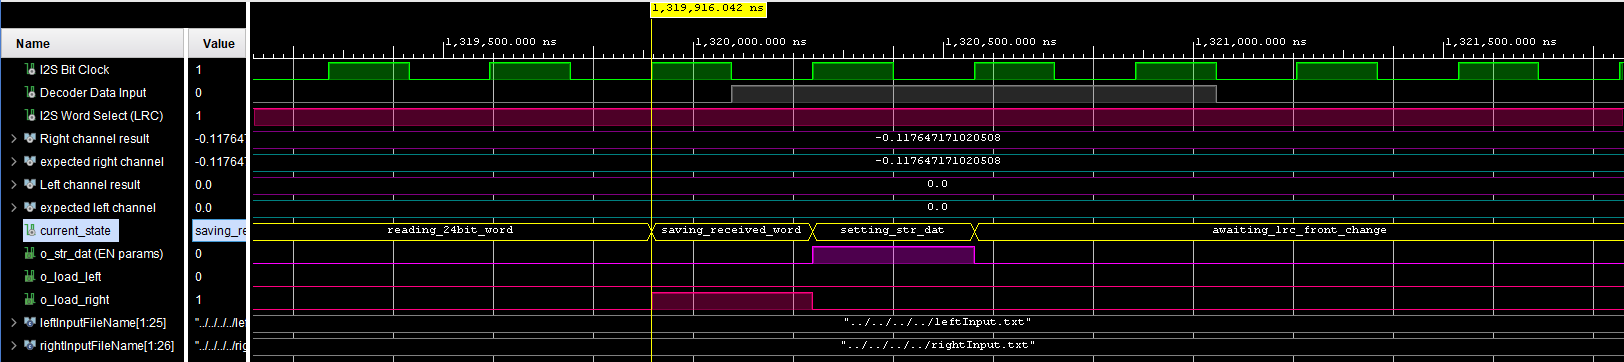
\includegraphics[width=\textwidth]{assets/chrono-m1-param-enable-reg-activation-return-await.png}
    \caption{Activation des registres et retour à l'état d'attente}
    \label{fig:chrono-m1-param-enable-reg-activation-return-await}
  \end{subfigure}
  \begin{subfigure}{.496\linewidth}
    \centering
    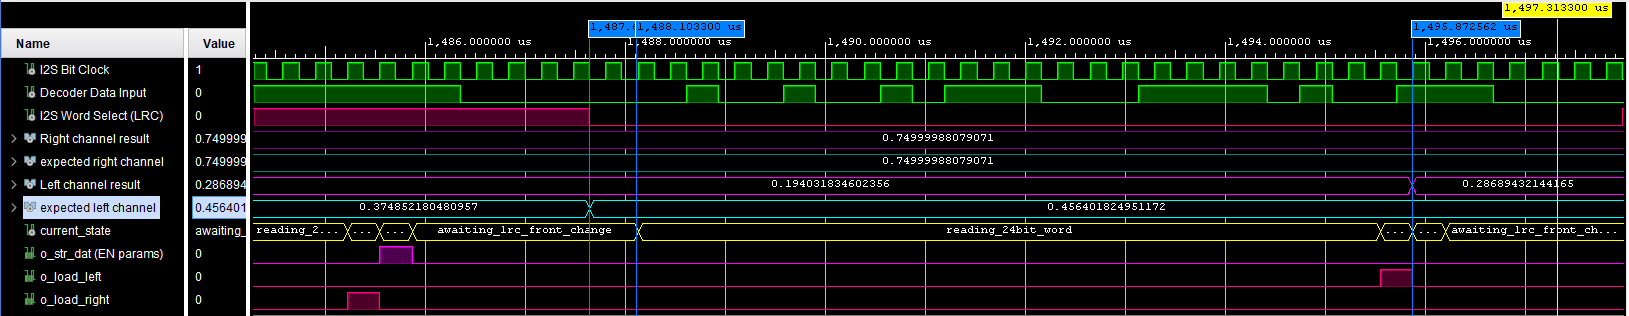
\includegraphics[width=\textwidth]{assets/chrono-m1-detect-change-LRC-save-output-to-channel.png}
    \caption{Détection du changement de LRC et enregistrement des données dans le canal approprié}
    \label{fig:chrono-m1-detect-change-LRC-save-output-to-channel}
  \end{subfigure}
  \begin{subfigure}{.496\linewidth}
    \centering
    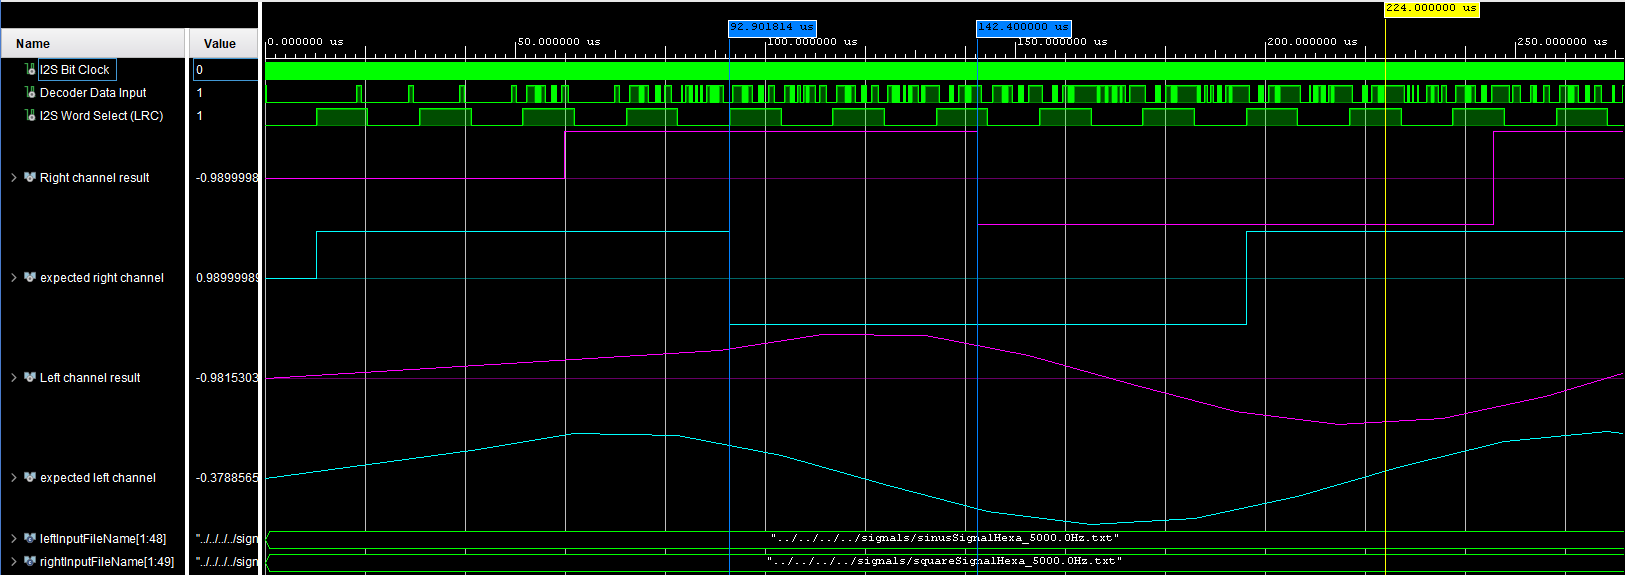
\includegraphics[width=\textwidth]{assets/chrono-m1-input-becomes-output.png}
    \caption{Conversion des données de sérial en entrée à parallèle en sortie}
    \label{fig:chrono-m1-input-becomes-output}
  \end{subfigure}
  \caption{Chronographes du module M1 sous différentes conditions}
\end{figure}





\note{votre lecteur ne connait pas votre démarche ni
pourquoi un tel résultat démontre le bon fonctionnement – vous devez l'expliquez brièvement.}

\note{Nous ne consulterons pas le dépôt de vos fichiers Xilinx (sauf
dans des cas particuliers) ce qui signifie que votre rapport doit être complet en lui-même.}

\subsection{Description du fonctionnement}

Le décodeur I2S détecte et extrait les échantillons stéréo (gauche et droite)
transmis en série par le CODEC audio via le protocole I2S. Son
fonctionnement repose sur une machine à états finis synchronisée par
l'horloge bit \verb|i_bclk|.\\

Le module débute dans l'état \verb|awaiting_lrc_front_change|, où il détecte
une transition sur le signal de sélection de mot \verb|i_lrc|. Lorsqu'une transition
est détectée, le compteur de bits et le registre à décalage sont réinitialisés,
et l'état passe à \verb|reading_24bit_word|.\\

Dans cet état, les bits sont captés en série à chaque front d'horloge et
décalés dans un registre. Une fois 23 bits reçus (le bit 0 étant le premier),
le décodeur passe à l'état \verb|saving_received_word|, où il déclenche le chargement
du mot complet dans un registre parallèle : vers \verb|o_load_left| si le mot
correspond au canal gauche (\verb|i_lrc| = 0), ou vers \verb|o_load_right| si
c'est le canal droit (\verb|i_lrc| = 1).\\

Finalement, l'état bascule à \verb|setting_str_dat| et active le signal \verb|o_str_dat| si le mot
appartient au canal droit. Ce signal sert à synchroniser les modules en aval,
comme les fonctions de calcul de puissance et de fréquence, qui ne s'appuient
que sur les échantillons du canal droit. Le système revient ensuite à l'attente
d'une nouvelle transition sur \verb|i_lrc|.


\todo{Validation via une simulation avec le banc de test fourni. Vous devez démontrer le
fonctionnement de vos modules au travers de simulations et expliquez en quoi vous
répondez aux spécifications. Faites bon usage des curseurs, formattage des données et
agrandissements pour appuyer vos propos.}
